\section{Performance Results}\label{sec:results}
We performed various experiments to measure the effectiveness of
\DataSeries{}' compression techniques, and then further compared other
types of data encoding and analysis tools for compression and
execution speed.  We first describe the experimental setup, then the
workloads, the benchmarks, and finally our results.

\subsection{Experimental setup}

The test-bed we used to perform most of the quantitative benchmarks for
this work was a cluster of 18 servers configured for batch processing of single server jobs.  Each server had one
or two dual core Opteron 280 2.4GHz processors.  Each processor had
64KB of L1 D-cache and 1024KB of L2 cache.  Additionally, each server
was configured with 4GB of main memory and could access a 10TB NFS
filesystem over 1Gb/s Ethernet, the underlying storage being RAID6 in
the form of HP MSA20 and MSA60 disk arrays.  The cluster was configured with
RedHat Enterprise Linux 4 and each server was running the 2.6.9 SMP
x86\_64 kernel version.  
% Results on a separate Xeon cluster showed
% similar results so we present only the Opteron cluster results.

%{\Large did we use any of the results from the XC cluster?  EA didn't think so CBM - NO}
%% We also tested our compression microbenchmarks on a second
%% cluster of 31 servers, each with four Xeon Pentium 4 2.8GHz
%% processors connected to the same NFS exported 10TB of storage.  Each
%% Xeon processor had 16K L1 D-cache and 2048K of L2 cache.  The Xeon
%% cluster servers were configured with Linux for High Performance
%% Computing running the 2.6.9 SMP x86\_64 kernel version.
%% 
%% Both clusters were managed with the Platform LSF~\cite{PlatformLSF}
%% batch cluster management software.

Finally, our comparison with C-Store~\cite{Stonebraker05} was performed
on a single machine with two dual-core Intel Pentium 4
3.0GHz Xeon processors, each with 16KB L1 D-cache and 2048KB L2 cache.
This machine was configured with 5 GB of RAM, running Debian Etch 4.0
with a 2.6.21.3 SMP-Bigmem Linux kernel.  The system also had a single
160GB Samsung HD160JJ Serial ATA hard drive.

\subsection{Data set descriptions}

Our data sets included the cello disk traces (``disk'') from HP Labs~\cite{SRT},
which we converted into \DataSeries{} from a custom binary format,
NFS traces collected from 
a busy enterprise file server (``NFS''), and file system call data
from~\cite{Soules05} (``system call''). 
Having three trace formats
each with very different extent types and associated data values provides
an indication of the performance and flexibility of \DataSeries{}
 in general.  For all
experiments to have a minimum of 10 extents with an extent size of
128MB (the largest we measured) all formats were transcoded into 1.2
GB (when uncompressed) files.  The smallest data set had six of these
files. 

For most of our experiments, the results from all three data sets were
similar, so we will only present detailed results and details on the
disk results. 
% NFS and system call datasets 
% were similar in shape to the disk results, so we present only the disk 
% results as the decisions made would be identical.  
We discuss our
use of the NFS traces in more detail in section~\ref{sec:discussion}, as 
it is by far our largest dataset ($\approx5$TB).

%\subsubsection{\textit{sar} data}

The disk traces contain entries that correspond to operating system
level read and write requests for blocks in a storage system.  Each
request contains three time fields (stored as doubles) describing when that request was
submitted to the device driver (enter\_driver), when the request
returned from the storage device (return\_to\_driver), and when the
request was returned to the calling process (leave\_driver).  
Additionally, the size (number of
bytes read/written) of each request, the logical volume identifier and
the device number are recorded as 32 bit integers. 
There are 28 boolean fields, eight 32-bit fields
 (including those mentioned above), two 64-bit fields and 
the three  double time fields.
 %{\Large EA: mention the other fields, at least the counts?}

The disk trace data set included six data files. For the \DataSeries{} 
analysis these files were compressed using lzf compression
to an average size of 320MB.  For the CSV analysis, they were
converted to CSV format using a \DataSeries{} to CSV converter.  For the
MySQL analysis, the files were further converted to the MySQL bulk-load
format and loaded into a single MySQL database table. The six files comprise
our ``small'' data set, while the combination of all six into a single
file comprise our ``large'' data set. The final data sizes
in all cases are shown in Table~\ref{table:dataSizes}. 
%{TODO: EA: why do we show LZF sizes?  That wouldn't be what someone would use}
% Used LZF because we were time constrained and LZO conversion is slow. - BM

%% \subsubsection{NFS traces}

%% Other bits about NFS moved into lessons.tex

%% The NFS traces used in the quantitative experiments contain entries
%% that correspond to NFS requests and replies in a production system
%% that handles up to 100TB of traffic per week.  Request types included
%% were attribute operations, mount operations, read-write operations,
%% and the statistics on packets which contained data.  
%% For example, the read/write request extent-type
%% included the the request or reply identifiers, byte offset and size of
%% the request and an NFS filehandle.  The NFS data set comprised twenty
%% 1.9GB data files.  The compression and CSV conversion techniques
%% were identical to those for the disk block traces.

%% \subsubsection{System call traces}
%% 
%% The system call data contains entries that correspond to
%% system call operations.  Several file system operations such as \texttt{link},
%% \texttt{mkdir}, \texttt{mknod}, \texttt{chmod}, \texttt{chown}, \texttt{open},
%% \texttt{close}, \texttt{read}, \texttt{write}, \texttt{remove}, and
%% \texttt{truncate} as well as process operations such as 
%% \texttt{fork}, \texttt{execve}, and \texttt{exit}
%% were recorded.  For example, for the \texttt{fork} system call, the
%% traces record process, user id and group identifiers, the return value of the
%% system call, the time the system call occurred in seconds and
%% microseconds, the child process identifier and the flags.  This data set
%% included twenty 1 GB data files.  The compression, CSV conversion and
%% database load techniques were identical to those for the disk block
%% traces.  Table~\ref{table:dataSizes} summarizes the trace data used in
%% both the compression microbenchmarks and analysis benchmarks.


%INSERT A TABLE INDICATING AVERAGE SIZES OF FILES FOR EACH TRACE SET AND
%FORMAT.


\begin{table*}[tbh]
\centering
\begin{tabular}{|c|c|c|c|}\hline
Trace Name & Avg. CSV Size & \DataSeries{} Size & MySQL Table Size\\
\hline
small disk trace & 2.3GB & 320MB & 1.5GB\\
big disk trace & 14GB & 1.9GB & 8.5GB \\
%% NFS data & 1.9GB & 272MB & untested \\
%% system call data & 1.2GB & 203MB & untested \\
\hline
\end{tabular}
\caption{ Trace data sizes in CSV, \DataSeries{} and MySQL formats.}
\label{table:dataSizes}
\end{table*}


%For the \DataSeries{}
%analysis these files were compressed using LZF compression to an
%average of 203MB.  For the CSV analysis, they were converted to CSV
%format using a \DataSeries{} to CSV converter.  For the MySQL analysis,
%the files were further converted to the MySQL bulk-load format and
%loaded into the MySQL database.

%For the \DataSeries{} analysis these
%files were compressed using LZF compression to an average of 272MB.
%For the CSV analysis, they were converted to CSV format using a
%\DataSeries{} to CSV converter.  For the MySQL analysis, the files were
%further converted to the MySQL bulk-load format and loaded into the
%MySQL database.

\subsection{Benchmarks}\label{sec:perfresults}

\DataSeries{} is optimized for, and performs very well on, queries which
 operate on scans of data or ranges of data.  We executed several
 encoding and decoding microbenchmarks to demonstrate the performance
 and tunability of \DataSeries{} as a trace storage and processing
 format.

Additionally, to provide a comparative analysis versus other known
 techniques for data processing, we generated nine related queries to
 run against a portion of the disk data set.  Unfortunately, C-Store
 could not perform the set of queries generated, so we performed a
 single simple query to compare C-Store and \DataSeries{}.

We performed experiments with data sets of two different sizes.  We
performed warm-cache experiments with the small data set since it
could fit in main memory.  We performed cold-cache experiments with
the large data set.

%% The bulk of the performance numbers for the competitive analysis were
%%  computed using 2.3GB of uncompressed disk data.  Since our clustered
%%  test machines all had 2GB or 4GB of system memory, all data fit into
%%  the file system buffer cache of the server.  We also ran a subset of
%%  queries on a 14GB (uncompressed) disk data set which represents 12
%%  days of disk traces to test out-of-core performance.

\subsubsection{Compression microbenchmark}

\DataSeries{} currently supports four different compression algorithms
(bzip2~\cite{BZIP}, gzip~\cite{GZIP}, lzf~\cite{LZF} and lzo~\cite{LZO}),
and an arbitrary extent size for record data.  Empirical knowledge and
algorithm author data seem to indicate that the algorithms are
optimized for different usages.  For example, bzip2 is commonly
believed to compress better than gzip, albeit more slowly.  Also,
all compression algorithms in common use today use a compression
window, giving the impression that compression ratio and perhaps
compression and decompression rate are optimized for files above a
certain size (i.e., the window size).  
We evaluated the compression ratio, compression rate, 
and decompression rate for each of these algorithms
using various extent sizes.

%{\Large say something about option for compression level, 9 for lzo, bz2,
%  6 for gz, na for lzf; need to say something about other choices.  Also
%should update legends to say lzo-9, gz-6, bz2-9}
Several of the compression algorithms (bzip2 and gzip)
have tunable parameters, which trade 
off compression rate for increased compression ratio.
We evaluated a range of settings for each of these algorithms.  
For the remainder of this section, we utilize bzip2 level 9 as
the representative for bzip2, and gzip level 6 as the representative
for gzip.  We found these levels provide reasonable tradeoffs
between the compression rate and ratio for each algorithm respectively.

Extent size determines the maximum window of data a compression
algorithm can look at.  For very small extent sizes, we expected to
see poor compression ratios because redundancy that would have been
within any algorithm's window size was artificially being blocked.
For very large extent sizes, we expected to see differentiation among
algorithms based on their window sizes.

The microbenchmark consisted of reading each \DataSeries{} file
%% in from its gzipped \DataSeries{} archive, 
and recompressing with the compression
algorithm under study.  The uncompressed data size was divided by the CPU time for the compression
operation  to compute {\em
Compression Rate}.  Next, the same file was decompressed and its
content thrown away.  The uncompressed data size was divided by the CPU time 
to compute the {\em Decompression Rate}.  
Finally, the compressed \DataSeries{} file size was
divided by the uncompressed \DataSeries{} file size to determine the {\em
Compression Ratio}.  The decompression and compression operations were
performed three times for each data file in each dataset.  All microbenchmark 
measurements were taken with checksum validation enabled.

%% \remark{Note that all \DataSeries{} files contain data transformations that reduce the size of the data.  The entire CMU data set contains 23GB of \DataSeries{} files compressed using GZip, while the raw binary compressed source data set is 45GB.}  

%% Several of the compression algorithms have tunable parameters that
%% trade off compression rate for increased compression ratio.  We
%% examine several settings for the bzip2 and gzip algorithms.

%% Figures~\ref{fig:bz2gzCompare}(a, b, c) show sample graphs of some
%% tradeoffs for different compression levels using the bzip2 algorithm.
%% There is a small difference in both compression ratio and
%% decompression rate for bzip2 level 1 versus 6 and 9.  All three data
%% sets have similar shapes for both decompression rate and compression
%% ratio, therefore for the remainder of the results bzip2 level 9 will
%% be presented as representative.  Figures~\ref{fig:bz2gzCompare}(d, e, f)
%% show similar curves for gzip, with slightly more differentiation in
%% compression ratio and decompression rate. Similar to bzip2, for all
%% three data sets, gzip has similar performance across different
%% compression levels and, due to space constraints, for the remainder of
%% the results gzip level 6 will be presented as representative of the gzip
%% algorithm.

%% \begin{figure*}[tbh]
%% \centering
%% \begin{tabular}{ccc}
%% \epsfig{width=1.5in, angle=270, file=graphs/amd/bz2-comRatio-srt.ps} &
%% \epsfig{width=1.5in, angle=270, file=graphs/amd/bz2-comRate-cmu.ps} &
%% \epsfig{width=1.5in, angle=270, file=graphs/amd/bz2-decomRate-cmu.ps} \\
%% (a) & (b) & (c)\\
%% \epsfig{width=1.5in, angle=270, file=graphs/amd/gz-comRatio-srt.ps} &
%% \epsfig{width=1.5in, angle=270, file=graphs/amd/gz-comRate-cmu.ps} &
%% \epsfig{width=1.5in, angle=270, file=graphs/amd/gz-decomRate-cmu.ps} \\
%% (d) & (e) & (f)\\
%% \end{tabular}
%% \caption{ Comparison of Compression Ratio, Compression Rate and Decompression Rate for bzip2 (a, b, c) and gzip (d, e, f) at compression levels 1,6, and 9: Compression Ratio for disk data; Compression and Decompression Rates for system calltrace 
%% Data. For this and all other results, error bars show 95\% confidence intervals.}
%% \label{fig:bz2gzCompare}
%% \end{figure*}

Next, we examined the performance of each algorithm, one metric at a time.
%% In some use cases, one metric will clearly be more valuable than others.
%% For example, 
For publishing traces or in archival situations the compression ratio will be the dominant
metric to consider.  Figure~\ref{fig:comRatio} shows the performance
of the tested compression algorithms on the disk trace data.
Bzip2 is the clear winner, achieving an average compression
ratio of about 10:1, for extent sizes 1 MB or larger.  
gzip and lzo performed similarly, achieving a maximum compression
ratio of about 6:1, for extent sizes larger than 128 KB.
lzf had the poorest compression ratio on this data set, achieving a
maximum compression ratio of about 3:1.
%% Although the compression ratios varied by data set, the relative ordering
%% was quite consistent across all of the data sets we tested.  As a result,
%% the results from the other data sets are not shown.

\begin{figure}[tbh]
%\centering
%\begin{tabular}{cc}
%\epsfig{width=2in, angle=270, file=graphs/amd/plotComRatio-cmu.ps} &
%\epsfig{width=2in, angle=270, file=graphs/amd/plotComRatio-nfs.ps} \\
%(a) & (b)\\
\epsfig{width=2in, angle=270, file=graphs/amd/plotComRatio-srt.ps}
%(c) \\
%\end{tabular}
\caption{ Compression ratio versus extent size results for disk trace data.}
\label{fig:comRatio}
\end{figure}


For online generation of \DataSeries{} files, the compression rate will
be the dominant metric to consider.  Figure~\ref{fig:comRates} shows the compression rates achieved by
each of the algorithms for the disk trace data.  
%% The relative
%% performance of the algorithms was similar across the datasets, and thus
%% the results for the other datasets are not shown.
lzf dominates in terms of compression speed, achieving 
a peak compression rate of ~90 MB/s, over four times
that of the next best algorithm (gzip).  The extent size appears to
have only a marginal effect on the compression rate achieved by the 
tested algorithms.  The ``no
compression'' (none) curve indicates the cost imposed
by the checksumming and data transforms.  The cost increases above 128KB 
as the data no longer remains in the L2 cache between the transform and
compression operations.
%% The overhead is quite significant
%% when the extent size is less than 128 KB, but less so for larger
%% extent sizes.

% Magic extent size only needs
%to be 98K to optimize for decompression rate.  Extent size should be
%set to approximately 1MB to optimize for compression ratio.  Extent
%size should be set to 64-98K to optimize for compression rate.

\begin{figure}[tbh]
%\centering
%\begin{tabular}{cc}
%\epsfig{width=2in, angle=270, file=graphs/amd/plotComRate-cmu.ps} &
%\epsfig{width=2in, angle=270, file=graphs/amd/plotComRate-nfs.ps} \\
%(a) & (b)\\
\epsfig{width=2in, angle=270, file=graphs/amd/plotComRate-srt.ps}
%(c) \\
%\end{tabular}
\caption{ Compression rate (logarithmic scale) versus extent size results for disk trace data.}
\label{fig:comRates}
\end{figure}

%% Figure~\ref{fig:decomRates} shows the decompression rates for the
%% tested algorithms.  As with the compression ratio and rate metrics,
%% the relative performance is consistent across the tested datasets,
%% so only the results from the disk traces are presented.
For trace analysis, the decompression rate will be the dominant metric to
consider, followed by compression ratio.
Figure~\ref{fig:decomRates} shows that the lzo algorithm has the
highest decompression rate, exceeding lzf while also achieving 
%$2\times$ 
2x more compression.  

%% Thus, this would be an excellent algorithm
%% to use for data which is read frequently (particularly if storage
%% space is not a major concern).  On our test sytem, lzo achieved
%% a decompression rate of almost 175 MB/s, for extent sizes between
%% 16 KB and 128 KB.  In second place is lzf, followed by gzip.  bzip2
%% achieved the poorest decompression rates, well below the other algorithms.

%For the decompression rate graphs, lzo dominates for decompression
%rate, but it costs you the worst compression rate of all algorithms.
%This would be an excellent algorithm to use for data which is read
%frequently, where space is not an issue.  

\begin{figure}[tbh]
%\centering
%\begin{tabular}{cc}
%\epsfig{width=2in, angle=270, file=graphs/amd/plotDecomRate-cmu.ps} &
%\epsfig{width=2in, angle=270, file=graphs/amd/plotDecomRate-nfs.ps} \\
%(a) & (b)\\
\epsfig{width=2in, angle=270, file=graphs/amd/plotDecomRate-srt.ps}
%(c) \\
%\end{tabular}
\caption{ Decompression rate versus extent size results for disk trace data.}
\label{fig:decomRates}
\end{figure}

A different view of the data can clarify these tradeoffs.
For online creation of \DataSeries{} files we care about the compression
rate and the compression ratio.
Figure~\ref{fig:comRateRatios} compares these metrics
with one point for each extent size.  The compression rate is shown
in log-scale because the different algorithms have vastly different rates.
This figure reinforces the previous graph showing that lzf dominates
with regard to compression rate, but gzip is a good tradeoff between
compression ratio and rate, sacrificing 10x the rate to get 2x
the compression.  bzip2 is useful if very high compression
ratios are desired, while lzo is dominated by all others on this graph.
Neither bzip2 nor lzo is likely to be suitable for online creation.

%% In some situations, multiple metrics may be important.  For example,
%% it may be desirable to compress the data reasonably well, but without
%% spending too much time doing so.  In this case, both the compression
%% ratio and compression rate metrics should be considered.
%% Figure~\ref{fig:comRateRatios} compares the four algorithms across
%% these two metrics, for the disk trace data (each subsequent point on a
%% line represents a larger extent size).  In this case we see that lzf
%% can achieve a compression ratio of about 3:1 while compressing the
%% data at approximately 90 MB/s.  The next best choice is gzip, which
%% achieves higher compression ratios, but at much slower rates.

\begin{figure}[tbh]
%\centering
%\begin{tabular}{cc}
%\epsfig{width=2in, angle=270, file=graphs/amd/plotComRateRatio-cmu.ps} &
%\epsfig{width=2in, angle=270, file=graphs/amd/plotComRateRatio-nfs.ps} \\
%(a) & (b)\\
\epsfig{width=2in, angle=270, file=graphs/amd/plotComRateRatio-srt.ps}
%(c) \\
%\end{tabular}
\caption{ Compression rate versus compression ratio results for disk trace data.}
\label{fig:comRateRatios}
\end{figure}

Figure~\ref{fig:decomRateRatios} compares the algorithms by the
compression ratio and decompression rate metrics.  This is important
for repeated analysis of data, a very common use case for
\DataSeries{}.  In this case, lzo dominates the other algorithms in
terms of decompression rate (\~175 MB/s), while still keeping a
reasonable compression ratio (\~6:1). lzo is strictly superior to lzf.
bzip2 achieves 
%$2\times$
2x increase in compression ratio, but at a 
%$10\times$
10x
reduction in decompression rate.  gzip achieves negligibly higher
compression ratios at a 
%$1.3\times$ 
1.3x reduction in decompression ratio.
Thus, gzip might only be considered if
lzo's compression time is too excessive.

\begin{figure}[tbh]
%\centering
%\begin{tabular}{cc}
%\epsfig{width=2in, angle=270, file=graphs/amd/plotDecomRateRatio-cmu.ps} &
%\epsfig{width=2in, angle=270, file=graphs/amd/plotDecomRateRatio-nfs.ps} \\
%(a) & (b)\\
\epsfig{width=2in, angle=270, file=graphs/amd/plotDecomRateRatio-srt.ps}
%(c) \\
%\end{tabular}
\caption{ Decompression rate versus compression ratio results for disk data.}
\label{fig:decomRateRatios}
\end{figure}

\subsubsection{Comparison with CSV, MySQL}\label{sec:compare}

\begin{figure*}[tbh]
\centering
\begin{tabular}{cc}
\epsfig{width=2in, angle=270, file=graphs/mysql-comparison.ps} &
\epsfig{width=2in, angle=270, file=graphs/mysql-comparison-14gb.ps} \\
(a) & (b)\\
\end{tabular}
\caption{ Query processing times for three sample queries using MySQL, our custom CSV engine, and \DataSeries{}.  Standard deviations for all data are smaller than 5\% of the average value: (a) 2.4GB disk trace File; (b) 14GB disk trace file.}
\label{fig:csvsqlcomp}
\end{figure*}

This set of benchmarks compared a hand-coded, type-specific \DataSeries{}
module (\DS{}-specific), a command line \DataSeries{} interface using \DS{}StatGroupByModule (\DS{}-generic), the
MySQL database, a custom application for parsing and processing Comma
Separated Value (CSV) files and C-Store, a research column-store database.  
These three additional
analyses give a sense for how well \DataSeries{} performs versus 
common alternatives. \footnote{These experiments were performed with lzf compressed files.  We plan to re-run the experiments with lzo compressed files and expect to see improved performance.}
% database
% software, versus handling data in ASCII text format and versus a state
% of the art column store.
%%%% state of the art is a bit strong isn't it? %%%%

While the authors are not database researchers, we felt using MySQL as
our representative database was a fair comparison because it is open
source (and thus an option for any researcher), provides the necessary
SQL parsing engine, is widely used for data analysis tasks, and has
reasonable performance.  It also provides an easy comparison point for
others to use when evaluating relative performance of their current
data analysis setup versus what they would gain by using
\DataSeries{}.  We believe for our experiments MySQL was suitably
tuned as the results from the large data set experiment were consistent with
the run being disk bound, and the results for the small trace file were
consistent with the run being CPU bound.

The first set of queries compute count, average, standard deviation, minimum and
maximum over the difference of each of the three time fields,
selecting for and grouping by each of the three non-time fields.  This
leads to nine possible queries.%, as shown in Table~\ref{table:queries}.
% These queries
%are shown in SQL for clarity.

%If we're keeping table:queries, this should be added to that

%\begin{table*}[tbh]
%\begin{tabular}{|l|lp{5.5in}|}\hline
%1 & \texttt{SELECT} & \texttt{device\_number, COUNT(*), AVG(leave\_driver - enter\_driver), STDDEV(leave\_driver - enter\_driver), MIN(leave\_driver - enter\_driver), MAX(leave\_driver - enter\_driver) FROM disk\_data GROUP BY device\_number;}\\ \hline
%2 & \texttt{SELECT} & \texttt{logical\_volume\_number, COUNT(*), AVG(leave\_driver - enter\_driver), STDDEV(leave\_driver - enter\_driver), MIN(leave\_driver - enter\_driver), MAX(leave\_driver - enter\_driver) FROM disk\_data GROUP BY logical\_volume\_number;}\\ \hline
%3 & \texttt{SELECT} & \texttt{bytes, COUNT(*), AVG(leave\_driver - enter\_driver), STDDEV(leave\_driver - enter\_driver), MIN(leave\_driver - enter\_driver), MAX(leave\_driver - enter\_driver) FROM disk\_data GROUP BY bytes;}\\ \hline
%4 & \texttt{SELECT} & \texttt{device\_number, COUNT(*), AVG(return\_to\_driver - enter\_driver), STDDEV(return\_to\_driver - enter\_driver), MIN(return\_to\_driver - enter\_driver), MAX(return\_to\_driver - enter\_driver) FROM disk\_data GROUP BY device\_number;}\\ \hline
%5 & \texttt{SELECT} & \texttt{logical\_volume\_number, COUNT(*), AVG(return\_to\_driver - enter\_driver), STDDEV(return\_to\_driver - enter\_driver), MIN(return\_to\_driver - enter\_driver), MAX(return\_to\_driver - enter\_driver) FROM disk\_data GROUP BY logical\_volume\_number;}\\ \hline
%6 & \texttt{SELECT} & \texttt{bytes, COUNT(*), AVG(return\_to\_driver - enter\_driver), STDDEV(return\_to\_driver - enter\_driver), MIN(return\_to\_driver - enter\_driver), MAX(return\_to\_driver - enter\_driver) FROM disk\_data GROUP BY bytes;}\\ \hline
%7 & \texttt{SELECT} & \texttt{device\_number, COUNT(*), AVG(leave\_driver - return\_to\_driver), STDDEV(leave\_driver - return\_to\_driver), MIN(leave\_driver - return\_to\_driver), MAX(leave\_driver - return\_to\_driver) FROM disk\_data GROUP BY device\_number;}\\ \hline
%8 & \texttt{SELECT} & \texttt{logical\_volume\_number, COUNT(*), AVG(leave\_driver - return\_to\_driver), STDDEV(leave\_driver - return\_to\_driver), MIN(leave\_driver - return\_to\_driver), MAX(leave\_driver - return\_to\_driver) FROM disk\_data GROUP BY logical\_volume\_number;}\\ \hline
%9 & \texttt{SELECT} & \texttt{bytes, COUNT(*), AVG(leave\_driver - return\_to\_driver), STDDEV(leave\_driver - return\_to\_driver), MIN(leave\_driver - return\_to\_driver), MAX(leave\_driver - return\_to\_driver) FROM disk\_data GROUP BY bytes;}\\ \hline
%\end{tabular}
%\caption{ Queries processed by \DataSeries{}, MySQL, and CSV engines.}
%\label{table:queries}
%\end{table*}

The compute time of these queries is relatively small so performance
should be dominated by the scan time of the data.  Ideally, only a
single scan of the data should be sufficient to compute the results
for these queries.  We attempted to optimize \DataSeries{}, MySQL and CSV
parsing to extract the fastest query response times possible.  

%% %THIS SHOULD BE ELSEWHERE!
%% \DataSeries{} provides two choices for executing the set of queries.  One
%% can write a small C++ program collecting the set of queries together
%% and computing them in a single pass of the data.  This has the
%% advantage that type checking is done at compile time and arithmetic
%% operators can directly access the elements of the data while the query
%% is running, speeding query execution time.  Alternatively, \DataSeries{}
%% provides for generic operators that provide run time type checking,
%% requiring a virtual function call on each arithmetic operation.
%% We used both techniques in our testing.
%% %END THIS SHOULD BE ELSEWHERE

We optimized \DataSeries{} by creating a type-specific version of the
queries, thereby eliminating the run-time type checking present
in the general purpose \DS{}StatGroupByModule.  We also disabled checksum validation to further improve performance.

We optimized SQL by minimizing the number of queries we issued. Instead of
issuing nine separate queries, we combined the queries when they were 
grouping by the same field, resulting in only three queries to compute
nine underlying SQL queries.

%% SQL syntax provides for grouping by a single field in a query.
%% Because there are three queries that group by each of bytes,
%% logical\_volume\_number and device\_number, SQL provides a natural
%% syntax for combining these queries together into groups of three by
%% each of the above fields.  However, without writing a query aggregator
%% for MySQL there does not seem to be an easy way to combine all nine
%% queries together to submit from a single client.  MySQL is a parallel
%% database however, so running the three triple queries or all nine
%% individual queries simultaneously using different connections to the
%% server should return results faster than running the queries
%% sequentially.

We optimized the CSV parsing by tuning the program, carefully parsing
the lines, caching conversions from strings to doubles, and only
converting fields that were being used.  Profiling showed we still spent 80\% of the
instructions in these operations with the remainder in the statistics
calculation.

\begin{figure*}[tbh]
\centering
\begin{tabular}{cc}
\epsfig{width=2in, angle=270, file=graphs/cstore-comparison-nohashes-walltime.ps} & 
\epsfig{width=2in, angle=270, file=graphs/cstore-comparison-nohashes-cputime.ps}  \\
(a) & (b)\\
\end{tabular}
\caption{ Query processing times for one simple query using C-Store and \DataSeries{}.  Standard deviations for all data are smaller than 5\% of the average value: (a) Wall clock time (sec); (b) CPU time (sec).}
\label{fig:cstorecomp}
\end{figure*}

%%  from strings to 
%% integers or doubles, and CSV files contain the data as ASCII text which must be parsed
%% into binary data before queries can be done on it.  However, all nine
%% queries can be answered with a single pass of the data once the data
%% has been parsed.

Each complex query was run seven times with the file system cache warm for the
2.3GB data set for each system.  The results are plotted in
Figure~\ref{fig:csvsqlcomp}(a).  The single query takes an average of
22.1 seconds with MySQL and 28.1 seconds with CSV, while \DataSeries{}
processes the same query in an average of 9.85 seconds, or 2-3X
faster.  Data processing rates are 2.3GB/22.1sec = 108MB/sec, 85MB/sec
and 243MB/sec respectively.  When three queries are combined, the
MySQL data processing rate drops to 2.3GB/32.1sec = 74.4MB/sec, CSV
drops to 64.7MB/sec while \DataSeries{} remained relatively unchanged at
242MB/sec. Per operation overhead with \DS{}-generic is much higher than \DS{}-specific, therefore, when all 9 queries are run, \DS{}-generic statistics computation dominates processing time, while \DS{}-specific runtime continues to be dominated by decompression.

Figure~\ref{fig:csvsqlcomp}(b) demonstrates the benefit of
the compression in \DataSeries{}. In this experiment the large disk trace is
used, so the trace must be read from disk rather than from the file 
system buffer cache.  As a result, the MySQL data processing rate has
dropped to 41.9MB/sec and CSV is at 40.9MB/sec, as both are disk bound. 
However, \DataSeries{} continues to process data at 243MB/sec
(because of the use of compression).  While investment 
in a faster disk subsystem could improve MySQL and CSV performance, 
\DataSeries{} is well balanced for modern desktops, compute clusters
and laptops.  A modern 1U server might have 2 or 4 drives and 8 cores, 
the number of drives is unlikely to increase, but the number of cores
continues to go up.

%% To understand {\em why} \DataSeries{} can process data so much faster, we
%% tried several different test configurations with \DataSeries{}.  First,
%% we uncompressed the \DataSeries{} files completely and recoded them to
%% have a very small extent size, 12KB in this case.  From the
%% decompression rate results, this should result in the highest possible
%% processing rate because an extent fits completely in L1 cache.  The
%% file size for this experiment was 6.9GB, and \DataSeries{} is able to
%% process the data at 45.4MB/sec.  This seems to indicate that disk I/O
%% is the bottleneck.  Compressing more heavily using lzo results in a
%% file size of 1.1GB which \DataSeries{} is able to process at 276MB/sec.
%  Finally, compressing using BZ2 significantly reduces file
% size on disk, resulting in a file of X.XGB but requires so much CPU
% time to decode that performance reduced to XXMB/Sec.

%% We conclude that because the system is disk bound, using compression
%% that does not significantly affect decompression rate improves
%% throughput significantly.  Another alternative would be to invest in
%% much faster disk hardware to process the data at whatever rate the CPU
%% could handle.  However, \DataSeries{} provides a software solution to this
%% balancing problem.  If the system has significantly faster CPU than
%% disk, a more CPU intensive compression algorithm can be employed to
%% achieve good throughput.

%% The CSV implementation was heavily tuned so that it only converts
%% values that are used and converts them at most once, but even so, 
%% profiling showed that it
%% was spending about 80\% of its instructions in the string manipulation
%% and conversion code.

\subsubsection{Comparison with C-Store}

As discussed in section~\ref{sec:related}, C-Store has recently been 
developed as a more efficient DBMS for read-mostly data.
Thus, we wish to compare its performance to \DataSeries{}.
Unfortunately, 
the open source C-Store implementation does not support any data type
except 32-bit integers, does not support expressions, and does not support multiple
aggregates in a single query.  Therefore, we could not compare C-Store
in the same manner that we evaluated MySQL and CSV.
Instead, for the C-Store comparison,
we chose a simple query that C-Store could support, the average I/O size in bytes grouped
by device number, on the large disk trace.
We used the default configuration of C-Store.
The simple query was run five times for each configuration of
\DataSeries{} and C-Store, with both a warm and cold file system cache.
We used the generic \DataSeries{} program and the type specific version
from the previous comparison. We also created a special case
type-specific version that only calculated the one statistic used
in our simple query.

The advantage of C-Store is that it is only reading the columns that
it needs in order to perform the calculation, whereas \DataSeries{}
has to read all of the columns.  Indeed,
Figure~\ref{fig:cstorecomp}(a) shows that when operating on all
columns, the warmed C-Store has a lower wall clock time
than any of the \DataSeries{} configurations.
C-Store's advantage when cold is quite small; this is a result of the
lack of (functioning) compression in C-Store.\footnote{C-Store is supposed to support
compression but we were unable to get it to work.}
However, if we
prune the \DataSeries{} file to just the 32 bit integer columns supported in
C-Store, the performance of \DataSeries{} can be better than C-Store.
In particular, the wall clock times for the type
specific and the one-statistic versions of the \DataSeries{} programs
both run faster than the C-Store queries for both the warm and cold
cases.  The CPU-time results shown in Figure~\ref{fig:cstorecomp}(b)
indicate that only the one-statistic version
of \DataSeries{} is using less CPU time; the much better wall clock time
shows the benefit of overlapping the decompression and statistics
calculations.  This result is somewhat surprising as
~\cite{VLDBCstoreTradeoffs} showed a column store needed to access
70-80\% of the columns in a row to use more CPU or wall clock time
than a row store, but we are showing that 25\% (2 of 8 int32 columns)
is sufficient for the row store to be faster.  This shows the
efficiency of the programming interface in \DataSeries{}.  As a
final comparison we
prune the files to just the columns used in the query.
In this case, the CPU time
for the one-statistic version of the \DataSeries{} program drops to
2/3 of the C-Store CPU time.

%% C-Store contains the data in files representing each column of the
%% data, opening the files when the query interface is bootstrapped.
%% Thus only columns needed by a query are scanned, potentially improving
%% performance when only a small subset of columns are needed (as is the
%% case for our simple query).

%% Three different configurations of \DataSeries{} were compared.  The
%% generic query engine, which in addition to the overhead to support
%% generics, also computes min, max, count, sum and sumsquared statistics
%% to derive mean and standard deviation; the typed query engine with the
%% same statistics; and the typed query engine computing only count and
%% sum to derive mean.  Additionally, the \DataSeries{} experiments were
%% run on three different source files.  One file, labeled 'all columns'
%% contains all of the disk trace data and is 14GB uncompresssed and
%% 1.1GB compressed using LZO.  The second file, labeled '32-bit columns'
%% contains the set of columns that C-Store is able to represent
%% (The open
%% source implementation of C-Store can only represent 32-bit fixed data,
%% no variable sized fields, and no other data sizes.)  
%% It is
%% 3.4GB uncompressed and only 129MB compressed using LZO.  
%% Finally, to
%% compare the data processing implementations of \DataSeries{} and
%% C-Store, the final file labeled 'query columns' contains only the two
%% columns in the query, and is 715MB uncompressed and 69 MB compressed.
%% C-Store results are repeated with each file for comparison purposes.
% We believe that '32-bit columns' result is the fairest comparison. 
% C-Store was compatible with only the 32-bit columns, and so is most
% comparable with the middle set of \DataSeries{} columns.

%% \DataSeries{} performs more slowly than C-Store when processing the
%% full set of columns.  Decompression overhead dominates the cost of the
%% operation in \DataSeries{}.  However, the '32-bit columns' portion of
%% Figure~\ref{fig:cstorecomp}(a) demonstrates that \DataSeries{} is
%% competitive over the set of columns C-Store can process, especially if
%% generic support and extra statistics calculations are removed from
%% \DataSeries{}.  Finally, the 'query columns' portion of
%% Figure~\ref{fig:cstorecomp}(a) shows how efficiently \DataSeries{} is
%% written compared with C-Store, as it computes more
%% complex statistics over the same two columns C-Store uses in less
%% time.

%% The open source C-Store implementation we used does not support
%% expressions, does not handle any data type except 32-bit signed
%% integers, and appears to be single threaded.  

%% \DataSeries{} can
%% support expressions, handles multiple data types including
%% variable-sized data, and is multi-threaded.  The performance of
%% multi-threaded pipelining is obvious in Figure~\ref{fig:cstorecomp}(b)
%% which shows wall clock time.  \DataSeries{} warm and cold performance
%% are very close, and CPU consumption monitoring indicated to us that
%% \DataSeries{} was computationally bound on two CPUs and could have
%% multiplexed more decompression to further improve performance.  This
%% is something we will consider in future work.  C-Store's cold
%% performance is blocked on I/O, and thus is outperformed in every case
%% by \DataSeries{} when operating on the '32-bit columns' or 'query
%% columns' files.  \DataSeries{} completes in 50\% of C-Store's warm
%% time when computing the same statistics over the same columns.

The limited functionality of the C-Store implementation make it
unusable for generic trace storage and analysis, but the results show
that some of the column store techniques to avoid processing un-needed
columns may benefit \DataSeries{} provided they can be implemented
without sacrificing the efficiency of the \DataSeries{}
implementation.  In our experience with \DataSeries{}, we usually run
multiple queries (different modules) at the same time when analyzing
data and the combination of those modules often accesses most of the
columns.  If this usage is common, the advantages of column oriented
storage would be reduced. 
%% In cases where only a subset of the columns are used repeatedly,
%% creating an interim data file that only contains the needed columns could
%% be done quickly, which would enable \DataSeries{} to achieve performance
%% similar to or better than C-Store.

%% Because \DataSeries{} provides tools for extracting relevant columns
%% and creating a new \DataSeries{} file with only those columns, the
%% advantage of C-Store when operating on a narrow set of columns is
%% removed.  Additionally, because C-Store cannot handle variable length
%% fields, or expressions, it is not usable as a reasonable storage or
%% query processing mechanism.

\subsection{Ellard Traces}

In an effort to experiment with using DataSeries to represent and
analyze traces generated by other people, we converted Daniel Ellard's
Harvard traces\ref{Ellard03} into DataSeries.  The Ellard traces
were originally stored as compressed text files, one record per line.
The first part of each line is a series of fixed fields, followed by a
set of key-value pairs, and finally some debugging information.  As
part of the tools, there is also a scanning program which reads the
trace files and outputs summary information for a trace.

Our evaluation came in two parts.  First, we wrote programs that
converted between the two formats.  The reversable conversion
guaranteed that we were properly preserving all of the information.
We found that the DataSeries files were on average 0.74x the size of
the original files when both were compressed using gzip.  Second, we
wrote an analysis program that implemented the first three examples in
the README that came with the tools.  We found that our analysis
program ran about 76x faster on those data files than the text
analysis program that came with the distribution.  
We also found that if we utilized lzo compression, which decompresses
more quickly than gzip,
our analysis program
ran about 107x faster, in exchange for slightly larger (1.14x) data files.
Other options in the space-time
tradeoff are described as part of the experiments.

\subsubsection{Conversion to and from DataSeries}

The conversion to DataSeries was interesting for two reasons.  First,
it stretched DataSeries in the direction of supporting many nullable
fields, which we had previously resisted going.  Second, it turned out
to be a case study in the difficulties posed by ad-hoc text formats.

DataSeries was designed to follow a relational database model.  As
such it supports null fields, although we have not put any special
optimizations in place to handle them (null fields were previously
just an extra boolean and a test).  While there was a slight space
penalty for having a few null fields, this penalty was mostly removed
by the compression algorithms.  However, when there are many null
fields, it could be much more space efficient to explicitly remove the
null values and create variable length rows before using a generic
compression algorithm.  We call this process null compaction.  We had
previously considered and decided against this feature because it
encourages people to choose schemas that do not follow normal form.
In the Ellard traces, this manifests as not knowning which columns
will be valid given a particular operation type when it is likely that
the operation type and valid fields are fixed.

In our initial conversion of the data, it appeared that the duplicate
elimination performed by the pack\_unique option would compensate for
the additional space used by storing a value for all of the fields.
However, once we had identified all of the fields we needed to store,
the naive implementation resulted in larger DataSeries files than text
files.  There were two options at this point, first, null compaction,
and second, normalizing the data design.  Normalizing the data design
would involve separating out the rows into multiple tables potentially
with keys to have a common and optional tables.  After further
consideration we decided that the most faithful representation would
be a single table, and hence to get small files we implemented null
compaction.

We implemented a reverse conversion program so that people could
continue to use existing scripts, and so we could verify that the
conversion worked properly.  This turned out to be very important, as
the files had a number of glitches in them.  This is a common problem
with under-specified text formats: it is very easy to generate a file
which appears to conform to a specification, but doesn't.  The same
problem can occur with XML, as it is easy to generate invalid XML.
Related to this problem is the lack of a specification; without a
specification, users have no idea what information may be present.
Similarly, in XML without a document type definition (DTD), it is
difficult to understand the meaning of a parsable document.  We solved
the problem of unparsable lines by introducing a ``garbage'' field
into the DataSeries output that stores unparsable lines.  We currently
have code that detects all of the unparsable lines, but if we had
known there would be as many as there were, we would have instead
written the code to throw an exception on parsing errors and store
unparsable lines as garbage.

We experienced a number of these problems in parsing and converting
the Ellard data.  We plan to make checksums (\texttt{sha1} and
\texttt{md5}) available so that people can validate they are working 
with the same input data we used.  We categorize these problems as 
follows:

% Move this so it shows up on same page as reference.
\begin{table*}[t]
\centering
\begin{tabular}{|c|c|c|c|c|c|c|}\hline
Trace Set & gz-64k  & gz-128k & gz-512k & lzo-64k & lzo-128k & bzip2-16M \\ \hline
overall   & 0.9459x & 0.8531x & 0.7721x & 1.1387x & 1.0437x & 0.76x   \\
deasna    & 0.9800x & 0.8856x & 0.7996x & 1.1535x & 1.0552x & 0.8064x \\
deasna2   & 1.0003x & 0.8976x & 0.8051x & 1.1680x & 1.0614x & 0.8148x \\
home02    & 0.9111x & 0.8204x & 0.7440x & 1.1252x & 1.0335x & 0.7084x \\
home03    & 0.9059x & 0.8170x & 0.7422x & 1.1197x & 1.0301x & 0.7073x \\
home04    & 0.8974x & 0.8094x & 0.7358x & 1.1148x & 1.0261x & 0.6979x \\
lair62    & 0.9663x & 0.8949x & 0.8271x & 1.1153x & 1.0427x & 0.8145x \\
lair62b   & 0.9859x & 0.8883x & 0.8009x & 1.1597x & 1.0579x & 0.8438x \\
\hline
\end{tabular}

\caption{Compression ratios for the different options.  The gz and lzo
columns are compared relative to the gzip compressed text files.  The
bzip2 results are compared to bzip2 compressed text files.  The
results exclude the 8 files with zero blocks in them.  The sizes after
the compression ratio is the extent size used for the DataSeries files.}

\label{table:ellard:compression}
\end{table*}


\begin{itemize}

\item {\bf Duplicate keys.}  The Ellard traces have key-value pairs on
each line.  We initially asumed that the keys were unique.  However,
we learned that this assumption is incorrect, as a subset of the keys
can occur multiple times on a single line.  Inspection of the code
that ships with the Ellard traces indicates it handles this case by
detecting the duplicate key and silently appending a ``-2'' to the
field name in the in-memory representation.  We translate these fields 
as \texttt{\_dup} to make them clearly separate from the Ellard 
translation of {\it field}2 for some duplicated fields.

\item {\bf Unknown keys.} There is no explicit list of the keys used
in the Ellard traces, hence we had to dynamically build up the list of
keys that could be present by attempting to parse a file and
generating an error if we found a new key.  The DataSeries files
include (as part of the extent type) the list of all unique fields
observed.  We later learned that except for the duplicate key issue
and the few keys with 2 on the end of the names, the key names follow
the xdr spec, so could be inferred from there.

\item {\bf Keys with identical meaning and different names.}  The
Ellard traces parse NFSv3 file handles as a field named \texttt{fh},
but NFSv3 commit file handles into a field named \texttt{file}.
Similarly, file names are parsed as \texttt{fn} for v2 and
\texttt{name} for v3, and offset is parsed as \texttt{offset} for v2
and \texttt{off} for v3. The DataSeries files document these
inconsistencies in a comment for that field.  We could have removed
the inconsistency, but that would have been less faithful to the
original files.  This inconsistency is present as a result of Ellard's
converter following the xdr spec which uses different names for fields
with the same meaning.  The intent was to make it easy to map the
traces back to the xdr, we would have chosen to make the field names
consistent to make it easier to write analysis.

\item {\bf Format changes.}  The Ellard traces document that at some
point they changed the semantics of the \texttt{acc} field from a
character to a bitmask.  To make conversion from DataSeries to the
text format work, we had to determine the date for the change so we
could generate different output depending on the date.  The DataSeries
files always use a bitmask, but if we had encountered this problem, a
version change would clearly indicate the format used in each file.
The earlier acc values are inaccurate and shouldn't be trusted, the
DataSeries files have a comment indicating the time at which the
switch occurred.

\item {\bf Format inconsistencies.} The Ellard traces document a
series of fixed fields at the beginning of each line.  However, for
the null operation, the reply format is missing one of those fixed
fields; we had to special case parsing null fields.  Similarly,
different operations print out the fields in different orders.  While
this is valid and correct, it meant we had to special case the
conversion from DataSeries to text to print fields in the appropriate
order.

\item {\bf Garbage times.} The Ellard traces specified that times were
in microseconds since the unix epoch, consistent with how NFS
represents these times.  In particular, times were printed as the
regular expression [0-9]+\\.[0-9]{6}, i.e. a series a digits, a period
and then 6 more digits.  Unfortunately, in a number of cases, the
lines did not match that format; 185 of these cases we explicitly
listed, and two numbers showed up sufficiently often that we checked
for them explicitly.  While the number of garbage times is a small
fraction of the total number of lines, it still is worrisome.  We also
subjected the times to a check that they were in a reasonable range of
9 or ten digits for the seconds.  We identified 17 special numbers
that we can't prove are invalid, but some of them are likely to be
network parsing errors; however since we couldn't tell, we parse them
as if valid.  The specific values can be found in the
\texttt{ellardnfs2ds.cpp} source file.

\item {\bf Garbage trailer.}  The Ellard traces end with some
debugging information that has been converted from numbers to XXX's in
the anonymous traces.  Unfortunately, when the line was short, the
cleanup for the trailer was done incorrectly and the debugging
information was left in.  Initially, it looked like the debugging
information was all identical for short packets, but later we found
some cases where it wasn't, so we passed it through as garbage.
Interestingly, the documentation says that the debugging fields can't
be removed because it would break scripts.  This is an advantage of a
format like DataSeries wherein analysis that don't need those fields
would not care if they were removed.

\item {\bf Non-data lines.}  A few lines started with ``XX Funny
line'' We pass these lines through as garbage.

\item {\bf Unknown errors.} There were 36 lines which had some sort of
random error in them.  Most of the errors look like a number of
characters were inserted or deleted at random combining or splitting
multiple lines.  A few of them look like the underlying packet data
was bad, but an output line was still generated as the stable field is
listed as `?'.

\item {\bf Zero blocks.} Eight of the compressed files have long
(multi-MB) blocks of null characters (`$\backslash0$') in them.  We
suspect this came from a toolchain error before we got the files, we
re-downloaded one of the files and verified that it had the block of
nulls in it.  This confused our parser since it saw a line that just
happened to not end with a newline, but thought it had reached the end
of the file as we were using \texttt{fgets}.  We eventually decided
not to try to translate these files, although in theory we could
update our program so that it would properly parse them, and pass them
through as garbage.

\end{itemize}

\subsubsection{Compression comparison}

Table~\ref{table:ellard:compression} shows the DataSeries compression results
relative to the original Ellard traces.  The compression difference
using bzip2 compression is slightly lower than with gzip, the
DataSeries files are 0.76x smaller than the text files compressed
using bzip2.  We compared the lzo files to the gzip compressed files
since for the text files compression with lzo would offer no benefit,
the files would be larger and the wall time for analysis would be the
same.  For gzip we tested with extent sizes of 64k, 128k and 512k.
For lzo, we tested with extent sizes of 64k and 128k.  We didn't
bother to calculate compression ratios for lzo-512k because the
performance is no better than gzip, and the compression would be
worse.  Interestingly, the ratios are not constant across the
different trace sets:

We have not investigated what causes the difference in the compressed
file sizes.  We have observed that for the small extent sizes
(64k/128k) the compressed extents are very small (5-10k), which means
that some of the DataSeries per-extent overhead may be contributing to
the larger size, as well as the compression algorithms may not have
enough data to even fill their window.

\subsubsection{Performance comparison}

For the performance comparison, we implemented a subset of the
analysis performed Ellard's \texttt{nfsscan} program. In particular one
that can perform the first three of the five example questions
presented in the EXAMPLES file that comes with Ellard's trace tools.
This analysis turned out to be very simple, it is just counting the
number of requests performed of each client of each type.  We chose to
implement this over the integer operation id, rather than the string,
and so wrote a short table that converted NFSv2 and NFSv3 operation
id's into a common space. The performance comparison was done using
DataSeries revision 61f07e212acb972da6c603bed82ab2ec5ca1b731 from
2008-01-21.

Our initial implementation did not perform as expected.  In particular,
we expected to see
the CPU utilization exceed 100\% during execution because the
analysis and the decompression steps were overlapped.  Further
investigation using \texttt{oprofile} indicated that the analysis module was
only using 4\% of the total CPU time; 96\% of the application's time
was going into decompressing the extents.  We therefore decided it was
time to implement parallel decompression so that we could take
suitable advantage of our multi-core machines.

The implementation on multi-core machines appeared as if it would be
straightforward, we implemented a standard pipeline, with one thread for
prefetching extents off disk, and $n$ threads for decompressing
extents, defaulting $n$ to the number of CPU cores.  Each stage in the
pipeline had a maximum memory capacity.

Experiments with this scheme indicated that the performance had high
variance.  After studying the problem we identified two issues.
First, the analysis thread could be pre-empted by a decompression
thread, and second, the thread decompressing the first extent in the
decompression queue could be pre-empted by any of the other threads.
Either of these situations could result in stalls in processing, and
instability in the performance.  Eventually we decided to detect
these two conditions, the second by noting that the first extent in
the decompression queue is not ready, and the current decompression
thread is working on an extent far down in the queue.  In either of
these two cases, the decompression thread will call \texttt{sched\_yield} to
try to get the more important thread running again.

This use of \texttt{sched\_yield} is an inferior solution because it
can result in many system calls that end up doing nothing, or simply
transfer us from running one thread that doesn't matter to a different
thread that doesn't matter.  With the existing threading interface,
the only other option to try would be to use priorities, however it is
not clear that priorities are sufficiently pre-emptable across CPUs to
have a useful effect.  If we were to extend the kernel threading
interface, there are two obvious possibilities for an improved
interface.  The first is what we call a directed yield, it would be a
variant of \texttt{sched\_yield}, but would specify a thread that should start
running, the call would transfer control to that thread if it is not
running, or do nothing otherwise.  The second possibility is process
local priorities, this would allow us to increase and decrease the
priorities dynamically during a run (which is currently not allowed as
threads usually can't increase their priority), and it would isolate
this process from other processes so that decreasing a thread's
priority would not cause other processes to run in preference to the
thread with lowered priority.  It is unclear which of these solutions
would work best, or how they could be made properly composable so that
in more complicated pipeline graphs the ``right thing'' can still
happen.

All of our experiments were performed on a DL365g1 with 8 GB memory,
2x 2.4GHz dual-core Opteron 2216 HE.  Data was stored on nfs.
Ellard's \texttt{nfsscan} program was run \texttt{zcat (or bzcat) $|$
nfsscan -t0 -BC -}, so we get separate times for the decompression and
nfsscan execution, but a single elapsed time.  The detailed
measurements can be found in the DataSeries distribution in
\texttt{doc/tr/ellard-details.tex}.

\begin{table*}
\centering
\begin{tabular}{|c|c|c|c|c|c|c|} \hline
            & mean     & mean       & mean     & CPU     & mean     & Wall time \\
algorithm   & user (s) & system (s) & CPU (s)  & speedup & wall (s) & speedup  \\ \hline
ellard-gz   & 537.58    &  7.80     & 545.38   &  1.0x   & 545.71   &   1.0x   \\
ellard-bz2  & 638.48    & 12.68     & 651.16   &  0.836x & 571.49   &   0.955x \\
\hline
ds-gz-512k  &  22.91    &  3.62     &  26.53   & 20.557x &   7.16   &  76.186x \\
ds-gz-64k   &  21.45    &  1.14     &  22.59   & 24.147x &   5.81   &  93.945x \\
ds-gz-128k  &  23.30    &  1.19     &  24.49   & 22.268x &   6.30   &  86.604x \\
\hline
ds-bz2-16M  &  94.38    & 11.82     & 106.20   &  5.136x &  27.66   &  19.732x \\
ds-lzo-64k  &  18.71    &  1.14     &  19.85   & 27.472x &   5.10   & 106.897x \\
ds-lzo-128k &  21.15    &  1.10     &  22.25   & 24.514x &   5.74   &  95.022x \\
ds-lzo-512k &  24.07    &  4.07     &  28.14   & 19.382x &   7.40   &  73.762x \\ \hline
\end{tabular}

\caption{Summary of performance results for the two analysis programs
operating on a variety of input files.  The analysis was run over the
anon-home04-011118-* files.  For the ellard \texttt{nfsscan} program
the text files were compressed with either gz or bz2.  For the
DataSeries \texttt{ellardanalysis} program, the dataseries files were
compressed with either gz, bz2, or lzo, and used various extent sizes
as specified.  CPU and wall time are both relative to ellard-gz.}

\label{tab:summary}
\end{table*}



We compare below the performance of running \texttt{nfsscan} either
with gzip or bz2 inputs, and the performance of running DataSeries
with bz2, gzip, and lzo inputs.  Interestingly, for the gzip inputs,
the scheduler chose to keep the gunzip and the \texttt{nfsscan}
processes on the same CPU.  For bzip2, it used different CPUs, which
meant that \texttt{nfsscan} ran somewhat slower, presumably because
the data had to be copied between CPUs, bzip2 has a larger block size,
and the buffering was insufficient to smooth out the difference.

Table~\ref{tab:summary} presents the summary results, showing the
impressive speedup and reduction in CPU time that can be achieved by
using DataSeries.  The different sizes specified after the compression
algorithm for the DataSeries rows are the extent sizes. 
The substantial increase in system time for dealing
with large extents for bzip2 is a result of glibc's use of mmap/munmap
for large allocations.  Every extent results in a separate pair of
mmap/munmap calls to the kernel and hence a substantial about of page
zeroing in the kernel.  The detailed measurements can be found 
in the DataSeries distribution in \texttt{doc/tr/ellard-details.tex}.



\subsection{1998 World cup traces}\label{sec:world-cup-1998}

The 1998 World cup traces\cite{ita08} are one of the largest
publically available web traces.  They were collected from the many
web servers for the 1998 World Cup games.  We converted the traces
from the special raw format used for them into DataSeries, and also
created a version of the {\tt checklog} program that comes with the
traces as a comparison point for analysis.  For these traces, we found
that conversion to DataSeries files were on average 0.93$\times$ the
size of the original files, and that the analysis program used about
YY$\times$ less CPU time and ran about ZZ$\times$ faster.
% YY = 1.5, ZZ = 2 on my laptop

\subsubsection{Conversion to and from DataSeries}

The conversion to and from DataSeries was quite straightforward.  The
traces use a simple fixed record format of 4 32 bit integers and 4 8
bit integers.  The integers are unsigned in the original format, but
since DataSeries only supports signed 32 bit integers, we converted
to a signed format, and convert backwards during analysis.  

As with most of our converters, we convert both backwards and forwards
to verify that the conversion was correct.  The conversion results
turned out to be very strange; while overall DataSeries compressed 2\%
better, some of the files ended up being smaller while others ended up
being larger.  Further examination identified five factors that were 
affecting the file size:

\begin{itemize}

\item {\bf Compression level}.  The original gzipped World Cup files were
compressed using {\tt gzip -6}, as that is the default compression
level.  DataSeries files default to {\tt gzip -9}.  We simply
re-compressed all of the original files as level 9.  However, this
points out the importance of defaults as people have been downloading
and using needlessly oversized files since they were released.

\item {\bf Endianness}.  The original World Cup files were stored 
in big-endian format.  DataSeries files are stored in the native
endianness of the host, which on x86 processors is little-endian.

\item {\bf Field order}.  The original World Cup files were stored
with the four 32-bit fields first and then the 4 8-bit fields.
DataSeries happened to store the files with all the 8-bit fields first
followed by the 32-bit ones.

\item {\bf Field padding}.  The original World Cup files included
no padding.  DataSeries padded the files to an 8 byte boundary, so
added in an extra 4 bytes of zeros to each record.

\item {\bf Relative field packing}.  The original World Cup files stored
the time field as absolute seconds.  DataSeries includes an option to
store fields calculated relative to the previous value.

\end{itemize}

Table~\ref{table:wc1998:compression} shows the overall compression of
the different options.  The \{le,be\}-\{bts,stb\}-gz files are the
original data files stored in little or big endian format (le/be) and
big to small or small to big (bts/stb) ordering.  The original traces
are be-bts-gz.  The DataSeries file without any options is ds-base,
and then options can be added on for reducing the field padding to the
maximum column size (mcs), packing the fields in big to small order
(bts), or packing the time field self-relative (tsr).

% plots and tables can be re-generated using graphs/wc1998/plot.hg

\begin{table}
\centering
\begin{tabular}{|c|c|c|c|}\hline

               &            & ratio to & ratio to \\
    dataset    & size (MiB) & ds-base & be-bts-gz \\
\hline							   
ds-mcs-bts-tsr & 7648.98  & 1.133         & 1.077         \\
ds-mcs-tsr     & 7722.78  & 1.122         & 1.067         \\
ds-bts-tsr     & 7890.12  & 1.098         & 1.044         \\
ds-tsr         & 8065.99  & 1.074         & 1.021         \\
le-bts-gz      & 8152.47  & 1.063         & 1.011         \\
ds-mcs-bts     & 8183.98  & 1.059         & 1.007         \\
be-bts-gz      & 8239.15  & 1.052         & 1.000         \\
le-stb-gz      & 8391.09  & 1.032         & 0.982         \\
be-stb-gz      & 8411.46  & 1.030         & 0.980         \\
ds-mcs         & 8423.56  & 1.029         & 0.978         \\
ds-bts         & 8439.72  & 1.027         & 0.976         \\
ds-base        & 8663.78  & 1.000         & 0.951         \\
\hline
\end{tabular}


\caption{Compression options for the data files sorted from the smallest 
to the largest.  Gzipped files can be stored little or big endian
(le/be) and small to big or big to small (stb/bts).  DataSeries files
can be stored with the fields padded only to the maximum column size
(mcs), with the fields stored big to small (bts), or with the time
field packed self relative (tsr). be-bts-gz is the original 1998 World
Cup trace format.}

\label{table:wc1998:compression}
\end{table}

\subsubsection{Original file compression experiments}

\begin{figure}
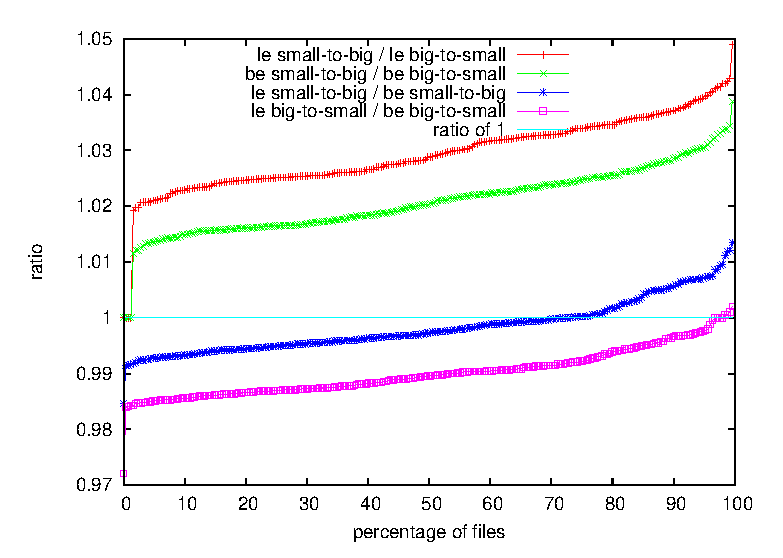
\epsfig{width=3.2in, angle=0, file=graphs/wc1998/reordering-options.ps}
\caption{Reordering options for the original data files.  
The data can be stored in little or big endian format (le/be); it can
also be stored with the small fields before the big ones or the
reverse (stb/bts)}
\label{fig:wc1998:original-data-reordering}
\end{figure}

Figure~\ref{fig:wc1998:original-data-reordering} shows the four
possible options for packing the data before compression in the
original data format.  Since the dataset includes some empty fields,
we always get some files that compress the same regardless of the
packing (to 20 bytes, the minimal gzip file size). 

The top two lines compare the small to big and big to small ordering
options holding the endianness constant.  Since both lines are
entirely positive, this shows us that we always prefer the
big-to-small ordering for this dataset (if the ratio is $>$ 1 then the
denominator is smaller and hence the preferrable choice), regardless
of endianness.  However, we note that changing the ordering makes more
of a difference if the files are little endian.

The bottom two lines compare the endianness choices holding the field
ordering constant.  Since the lines are mostly below zero, we in
gneneral prefer the little endian files to the big endian files, and
the preference is more pronounced for the big-to-small ordering.

\subsubsection{DataSeries file compression experiments}

The first DataSeries graph looks at the overhead imposed by the
DataSeries file format.  For this experiment, we pruned out the 5 tiny
files (4 empty, and 1 $<$4k compressed) in the dataset as DataSeries
imposes a large overhead on very tiny files since it includes the type
information in each file.  In particular, for an empty file, the
overhead is about 80x as at DataSeries files are 1.6k and the original
files are 20 bytes.  Figure~\ref{fig:wc1998:ds-overhead} shows
the overhead imposed by DataSeries with both the big-to-small and the
small-to-big orderings for the files, and using $10^6$ byte extent
sizes.  We can see that DataSeries imposes a 0.2\%-0.5\% overhead on
the files if the underlying data is identical.  We manually verified
that a few files were in identical except for the type extent at the
beginning of the file, the extent headers that occurred at the middle
of the files, and the trailer at the end.

\begin{figure}
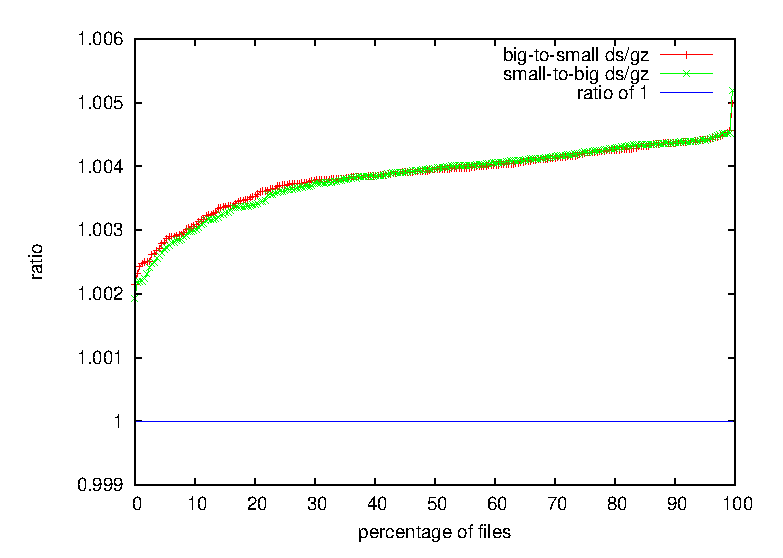
\epsfig{width=3.2in, angle=0, file=graphs/wc1998/ds-overhead.ps}
\caption{Overhead imposed by DataSeries. The record format is constrained
to be identical to the original data.  DataSeries imposes a
0.2\%-0.5\% overhead.}
\label{fig:wc1998:ds-overhead}
\end{figure}

The second graph shown in figure~\ref{fig:wc1998:ds-opts-1} looks
at the effect of the field packing (mcs) and field ordering (bts)
options for DataSeries.  We compare the file sizes measured by turning
on each of the options individually, and then both at the same time.
The results are much as would be expected; eliminating the extra
padding (mcs) gives us a flat 2-3\% compression improvement.
Switching to big-to-small (bts) field ordering gives a 1-4\%.  The
options combine to give us a 5-7\% compression improvement over the
base DataSeries case.  The one oddness is the couple of points that
are below 1.  These come from the empty files.  We changed the options
to the packing by changing the XML option from pack\_* to xack\_* so
as to minimize the change in the size of the type extent.  However,
having all three options specified as xack\_* compresses slightly
better (4 bytes) than having one or two options as pack\_* and the
others as xack\_*, resulting in the negligably below 1 ratio.

\begin{figure}
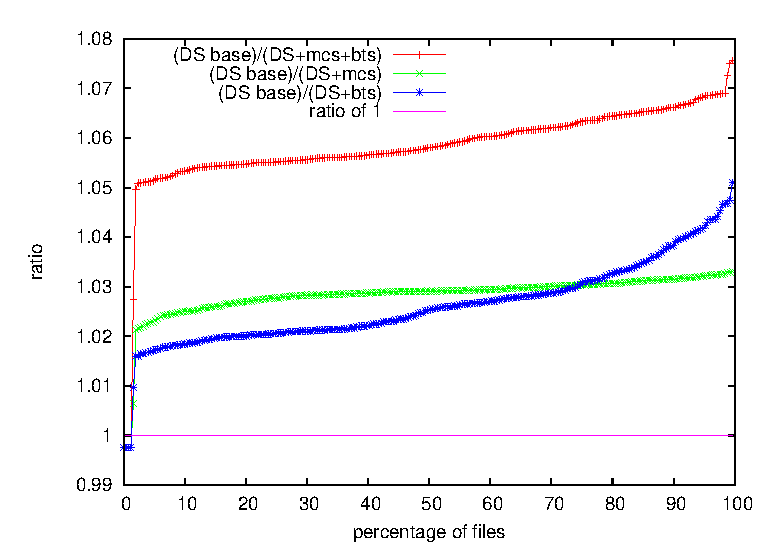
\epsfig{width=3.2in, angle=0, file=graphs/wc1998/ds-opts-1.ps}
\caption{Turning on the field compaction (mcs) and ordering (bts) options 
in DataSeries.  The compression options are mostly independent, so the
resulting compression of turning both on is multiplicative.}
\label{fig:wc1998:ds-opts-1}
\end{figure}

The third graph shown in figure~\ref{fig:wc1998:ds-opts-2} looks
at the effect of the time self-relative packing option and then
combines it with the field packing (mcs) and field ordering (bts)
options.  Time self relative gives a much more substantial improvement
in some cases -- by itself it can give a 20\% compression improvement.
However it does not operate nearly as independently as the first two
options, in particular turning on both bts and mcs packing is not much
of an improvement over just mcs packing.

\begin{figure}
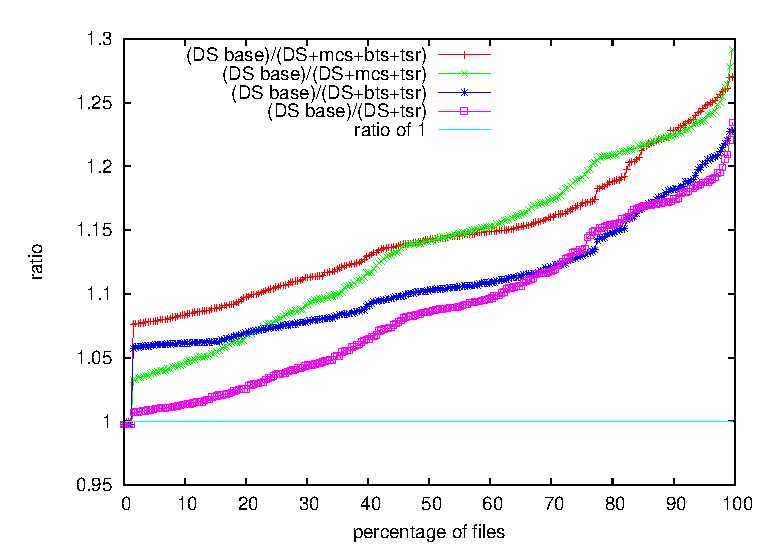
\epsfig{width=3.2in, angle=0, file=graphs/wc1998/ds-opts-2.ps}
\caption{Turning on the time self-relative (tsr) option and then the 
field compaction (mcs) and ordering (bts) options in DataSeries.  
With time self-relative packing, the options are no longer independent, 
and overall time self-relative gives a much more substantial improvement 
than the other options.}
\label{fig:wc1998:ds-opts-2}
\end{figure}

The fourth graph shown in figure~\ref{fig:wc1998:ds-opts-3} looks at
just the effect of turning on the big-to-small packing option with the
field compaction (mcs) and time self-relative (tsr) options already
turned on.  This graph shows why the benefit of big-to-small is so
minor once the other options are on.  The big-to-small option
interferes in some cases with the time self-relative option.  This
figure leads to the idea that different extents could be packed using
different field orderings as in DataSeries, each extent boundary could
be stored in different ways.

\begin{figure}
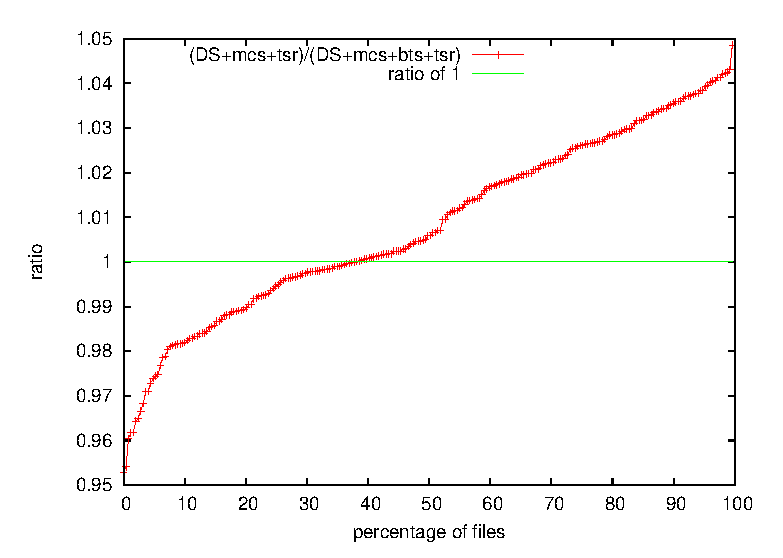
\epsfig{width=3.2in, angle=0, file=graphs/wc1998/ds-opts-3.ps}
\caption{Comparing just the field ordering option (bts) with both the
time self-relative (tsr) and field compaction (mcs) options enabled.
Packing big to small is a win, but not by much.}
\label{fig:wc1998:ds-opts-3}
\end{figure}

The fifth graph shown in figure~\ref{fig:wc1998:ds-size-cmp} looks at
whether or not there is any size correlation to the improvment
provided by the compression options.  Visually the graph shows no
significant correlation between size and compression ratio as the
values are just scattered within a range.

\begin{figure}
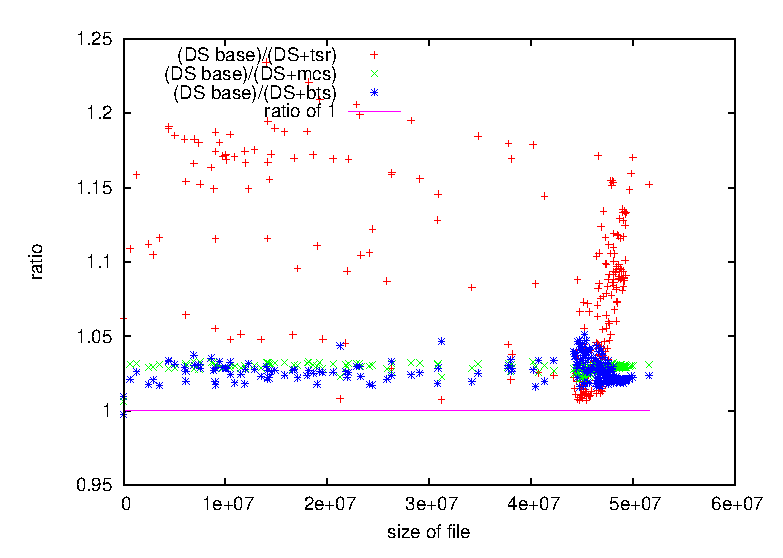
\epsfig{width=3.2in, angle=0, file=graphs/wc1998/ds-size-cmp.ps}
\caption{Determining if any of the compression options correlate with
size of the file.  Visually they do not appear to.}
\label{fig:wc1998:ds-size-cmp}
\end{figure}

\subsubsection{Compression conclusions}

The work in this section showed that the field compaction option had a
small but consistent effect on the compressibility of the data.  We
would recommend that any extent type that does not have any 8 byte
fields always turn on this option.  In fact, the option could be
turned on in general, but it will have no effect (other than consuming
a small amount of space in the extent type) if there are 8 byte fields
in the record type, or if the record size is otherwise a multiple of
8.

The work in this section also shows that field ordering can have a
substantial effect on the compressibility of an extent.  On every
extent boundary, the fields that access the extent get a chance to
re-calculate their offsets into the data.  This means that for graphs
like figure~\ref{fig:wc1998:ds-opts-3} we could in theory make it so
that all files are compressed as well as just having the mcs+tsr
options enabled.  Indeed, just choosing a per-file field ordering that
would match the best ordering for the file would improve the
compression.  However, we could potentially do even better as each
extent in a single file could choose the best ordering.  Moreover, we
have only tested a subset of the possible ordering options.  For this
dataset, there are actually $5!*4!$ possible orderings that don't
introduce additional padding.  This comes from there are 5 32-bit
units (4 actual and 4 8-bit) that could have any order, and then the 4
8-bit values could be ordered in any order.  We hypothesize that
correlations between fields will correlate with the amount of
compression that could be achieved, and hence it may be possible to
work out much better field orderings without evaluating an exponential
number of values.

\subsubsection{Analysis performance}

We re-implemented the {\tt checklog} program that comes with the 1998
World Cup traces.  That program calculates a couple of the values in
multiple ways.  We duplicated this calculation because we wanted the
programs to be comparable, even though performing the calculation is
unnecesary. When running the program we found that the DataSeries
implementation ran ZZ$\times$ faster.  This result was expected as the
analysis performed was fairly simple, and as DataSeries used multiple
CPUs for decompression, it was able to run faster.  However, we also
found that the implementation used about YY$\times$ less CPU.  This
was unexpected given that DataSeries was using a virtual function call
for every row, and was having to process the extents separately.  We
examined the CPU utilization using oprofile and valgrind and found
that the original code had three problems:

\begin{itemize}

\item {\bf Non-integrated decompression}.  The {\tt checklog} program 
used a separate process to perform the decompression, this led to
slightly increased system time to pass the data over the pipe.

\item {\bf Very slow byte-swapping routine}.  The {\tt checklog} program
had to byte-swap every record, and the implementation used for
byte-swapping was very slow.  Moreover, the implementation copied the
data rather than doing the byte-swapping in-place, further increasing
the overhead.

\item {\bf Slow per-record fread}.  The {\tt checklog} program called 
fread for each record.  While we didn't expect this to be slow, it
turned out that the implementation is slow, and so calling fread for
each record is a poor choice.

\end{itemize}

While we could re-implement {\tt checklog}, it doesn't seem
particularly valuable.  The expected end result would be that the
checklog program would use less CPU time than the DataSeries program,
but would use more wall-clock time because there is no easy way to
parallelize the reading of the underlying files.


